\section{Dataset Overview and Representation}

The dataset is constituted of $5$ columns, with meaning shown in Table \ref{tab:variable_overview}. And Figure \ref{fig:single-data-analysis} illustrates the distributions of all variables.

In Figure \ref{fig:single-data-analysis}, it is clear that $y$ is left-skewed. We consider setting \begin{equation}
    y' = \log^2 y
\end{equation} to fix the skewness of the response variable. Equation 

\begin{figure}
    \centering
    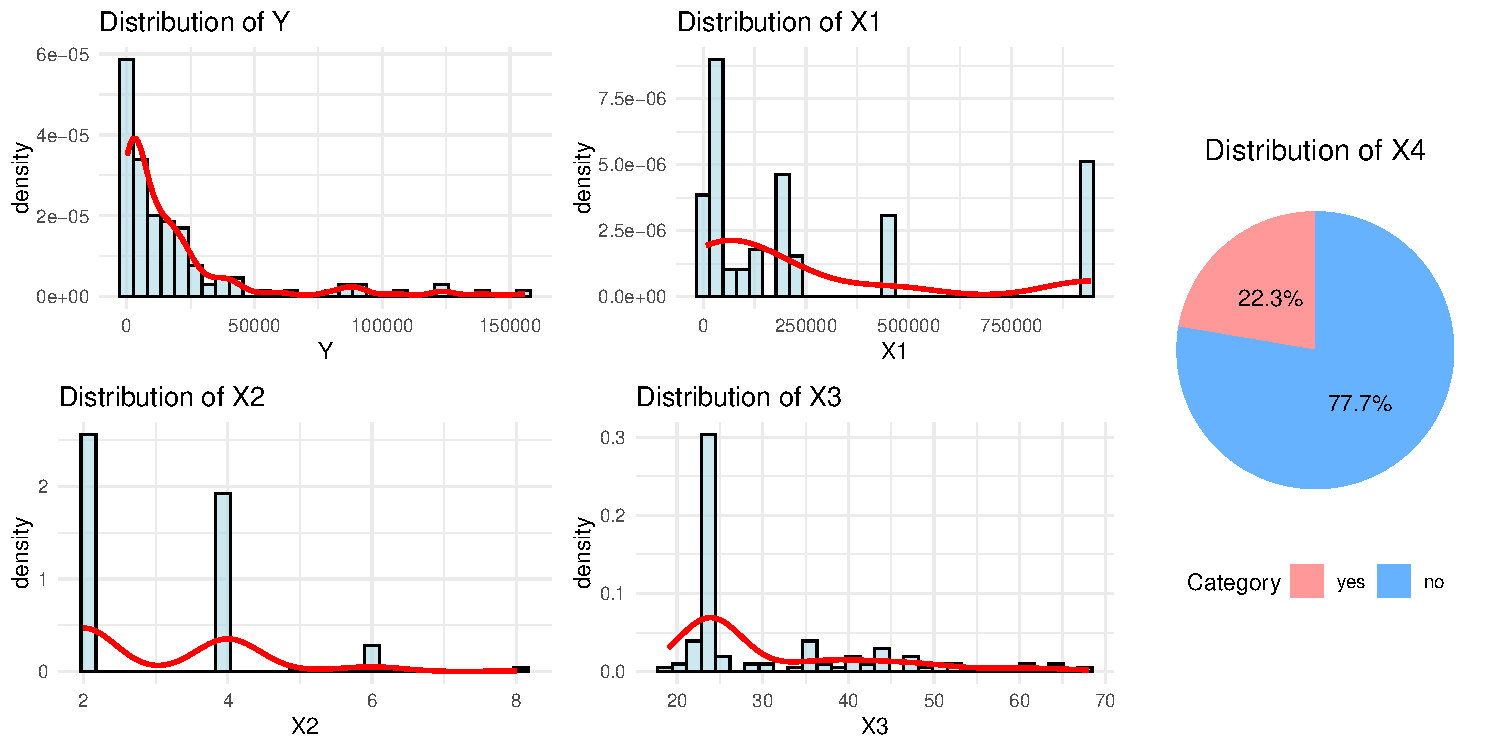
\includegraphics[width=1\linewidth]{figures/single_data_analysis}
    \caption{Distribution of the Variables}
    \label{fig:single-data-analysis}
\end{figure}

\begin{table}[t]
    \centering
    \begin{tabular}{c|l|l}
    \toprule
        \textbf{Columns} & \textbf{Meaning} & \textbf{Type}\\
        \midrule
        $y$ & Annual average daily traffic (AADT) & Continuous\\
        $x_1$ & Population of county in which road section in located & Discrete\\
        $x_2$ & Number of lanes in road section & Discrete\\
        $x_3$ & width of road section (in feet) & Continuous\\
        $x_4$ & Whether there is control of access to road section\tablefootnote{ $x_4 = 1$ means access control; $x_4 = 2$ means no access control} & Binary\\
    \bottomrule
    \end{tabular}
    \caption{Overview of the Variables}
    \label{tab:variable_overview}
\end{table}

In further analysis, we will use $y'$ as the response variable. To predict the value of $y$, we can easily do inverse transformation $y = \exp{\sqrt{y'}}$ to get the result.


Similarly, to fix the skewness of $x_1$, transformations are performed to $x_1$ with
\begin{equation}
x_1' = \sqrt{x_1}
\end{equation}

\begin{figure}
    \centering
    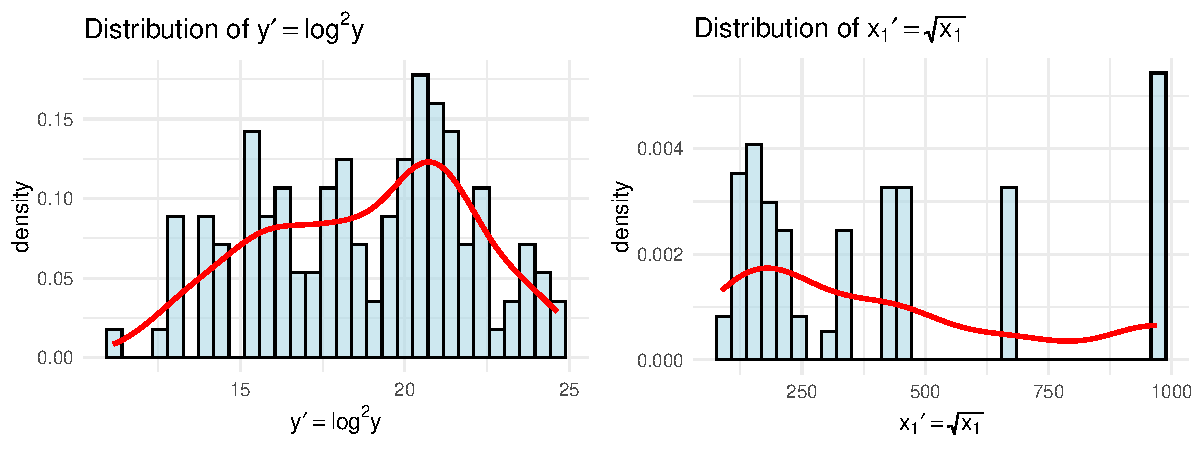
\includegraphics[width=1\linewidth]{figures/transformed_variables}
    \caption{Distribution of variables after transformation}
    \label{fig:transformed_variables}
\end{figure}

Figure \ref{fig:transformed_variables} shows the distribution of $y'$ and $x_1$, it can be seen that the distributions of $y'$ and $x_1'$ are relatively uniform compared with the original $y$ and $x_1$.

Although \( x_2 \) and \( x_3 \) also have some skewness, considering that they are integers\footnote{Although \( x_3 \) is defined as a continuous variable, it consists entirely of integers in the dataset.} with a small range in the dataset, applying a transformation may not be useful. We have decided not to transform them for now.

% For easier representation, we define the predictor as

